%!TEX root = art-in-machine-learning.tex

\section{Image Data}\label{sec:images}%

\subsection{Google DeepDream}\label{subsec:google-deepdream}%
The gradient descent algorithm which optimizes most of the parameters in neural
networks is well-understood. However, the effect it has on the recognition
system is difficult to estimate. \cite{inceptionism2015} proposes a technique
to analyze the weights learned by such a network. A similar idea was applied
by~\cite{vondrick2013hoggles}.

For example, consider a neural network which was trained to recognize various
images like bananas. This technique turns the network upside down and starts
with random noise. To analyze what the network considers bananas to look like,
the random noise image is gradually tweaked so that it generates the output
\enquote{banana}. Additionally, the changes can be restricted in a way that the
statistics of the input image have to be similar to natural images. One example
of this is that neighboring pixels are correlated.
\goodbreak
Another technique is to amplify the output of layers. This was described
in~\cite{inceptionism2015}:\nobreak%
\begin{displayquote}
We ask the network: \enquote{Whatever you see there, I want more of it!} This
creates a feedback loop: if a cloud looks a little bit like a bird, the network
will make it look more like a bird. This in turn will make the network
recognize the bird even more strongly on the next pass and so forth, until a
highly detailed bird appears, seemingly out of nowhere.
\end{displayquote}

\begin{figure}[ht]
    \centering
    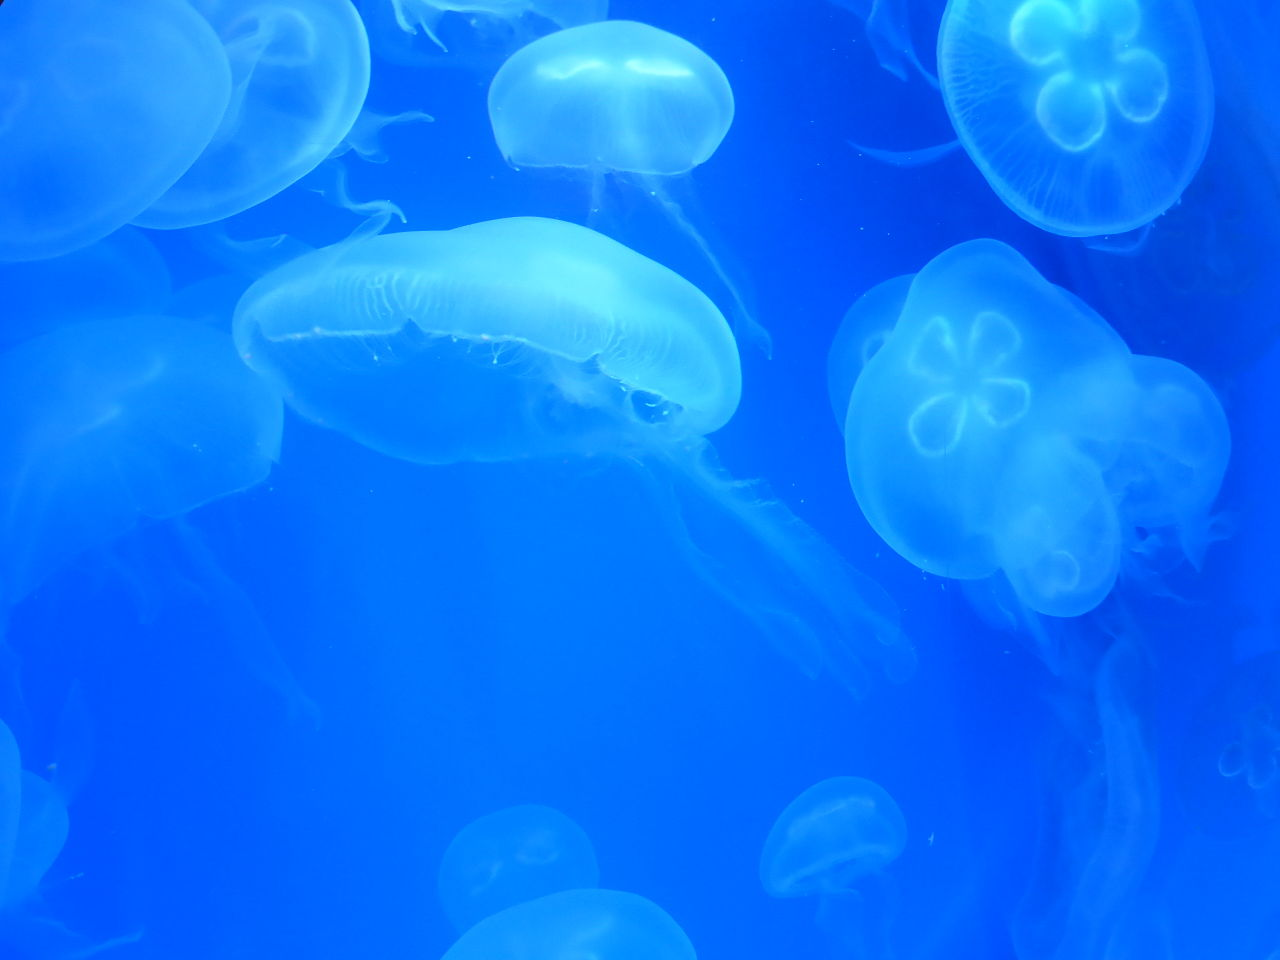
\includegraphics[width=0.45\textwidth]{figures/DeepDream/Aurelia-aurita-3/Aurelia-aurita-3.jpg}
        \label{fig:Aurelia-aurita-3-original}
    \caption{Aurelia aurita}
\end{figure}

\begin{figure}[ht]
    \centering
    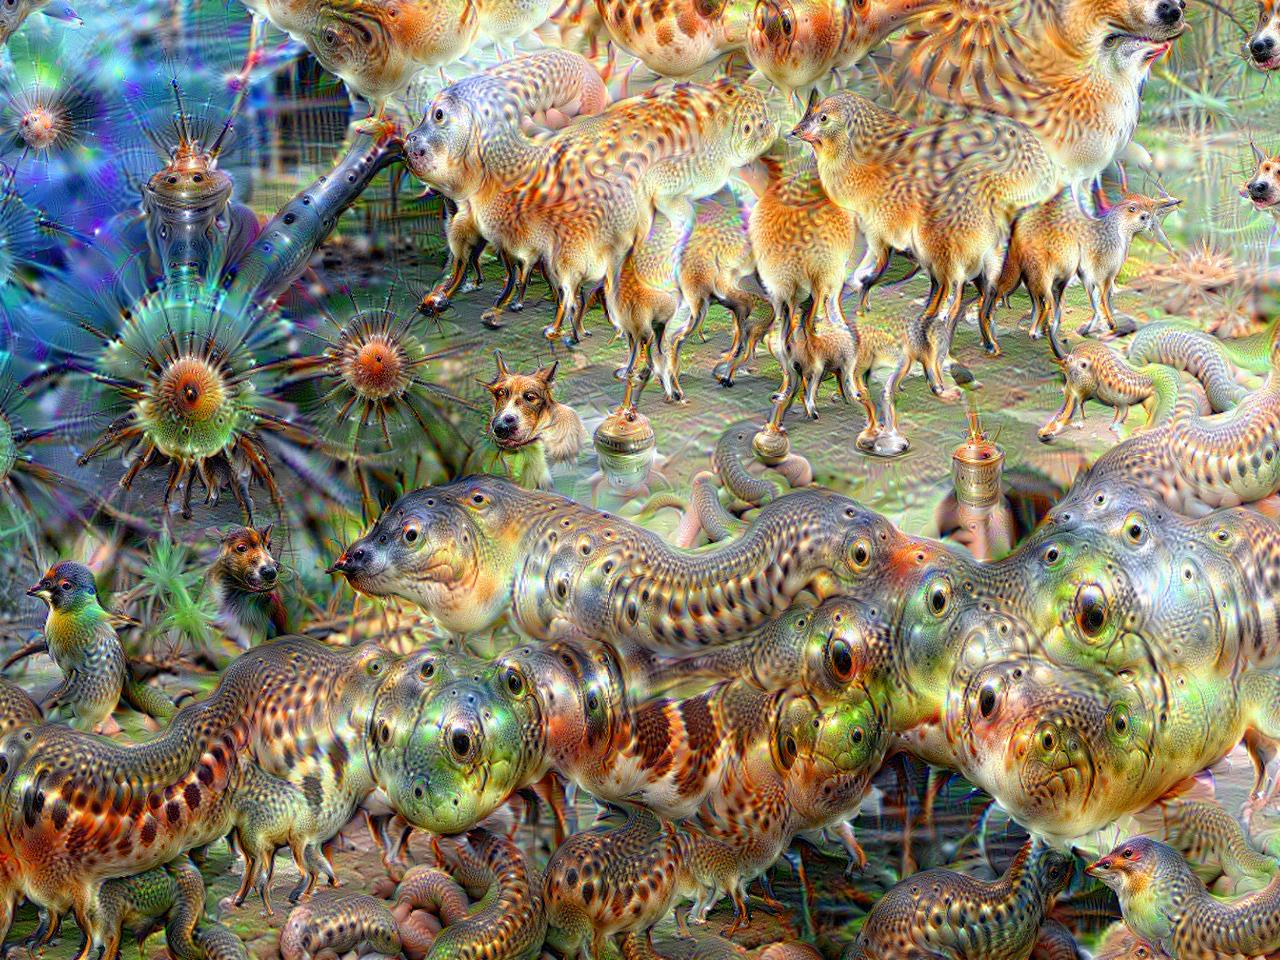
\includegraphics[width=0.45\textwidth]{figures/DeepDream/Aurelia-aurita-3/0099.jpg}
        \label{fig:Aurelia-aurita-3-100}
    \caption{DeepDream impression of Aurelia aurita}
\end{figure}

The name \enquote{Inceptionism} comes from the science-fiction movie
\enquote{Inception}~(2010). One reason it might be chosen is because neural
networks are structured in layers. Recent publications tend to have more and
more layers. The used jargon is to say they get \enquote{deeper}. As this
technique as published by Google engineers, images generated by this are called
\textit{Google DeepDream}.

It has become famous in the internet. (TODO: Reddit)
Images and videos published by the Google engineers can be seen
at~\href{https://goo.gl/Bydofw}{https://goo.gl/Bydofw}. TODO: Add own images.


\subsection{Magic The Gathering card creation}

TODO: \href{http://nerdist.com/what-happens-when-artificial-intelligence-makes-magic-the-gathering-cards/}{source}


\subsection{Caption generation}
Generating captions for images can be seen as a creative task, too. Interesting
captions don't only describe what one can obvioulsy see on the image, but also
interpret the image to a certain degree.

TODO: Show example.


\subsection{Artistic Style Imitation}
A key idea of neural networks is that they learn different representations of
the data in each layer. In the case of \glspl{CNN}, this can easily be
visualized as it was done in various papers (TODO: Cite). Usually, one finds
that the network learned to build edge detectors in the first layers and more
complex structures in the upper layers.

Gatys, Ecker and Bethge showed in~\cite{gatys2015neural} that with a clever
choice of features it is possible to separate the general style of an image in
terms of local image appearance from the content of an image. They (TODO:
untermauern) their point by applying the style of different artists to an
arbitrary image of their choice.

This artistic style imitation can be seen itself as creative work.

(TODO: Apply \href{http://gitxiv.com/posts/jG46ukGod8R7Rdtud/a-neural-algorithm-of-artistic-style}{http://gitxiv.com/posts/jG46ukGod8R7Rdtud/a-neural-algorithm-of-artistic-style} and add images)



TODO: \cite{shih2014style} \href{http://gitxiv.com/posts/eoxDf59kBz87tvkX3/style-transfer-for-headshot-portraits}{http://gitxiv.com/posts/eoxDf59kBz87tvkX3/style-transfer-for-headshot-portraits}


\subsection{Drawing Robots}
Patrick Tresset and Frédéric Fol Leymarie created a system called AIKON
(Automatic IKONic drawing) which can automatically generated sketches for
portraits~\cite{tresset2005generative}. AIKON takes a digital photograph,
detects faces on them and sketches them with a pen-plotter.

Tresset and Leymaire use $k$-means clustering~\cite{1017616} to segment regions
of the photograph with similar color which, in turn, will get a similar
shading.

Such a drawing robot could apply machine learning techniques known from
computer vision for detecting the human. It could apply self-learning
techniques to draw results most similar to the artists impression of the image.
However, the system described in~\cite{tresset2005generative} seems not to be a
machine learning computer program according to the definition by Tom
Mitchell~\cite{Mitchell97}.
